\subsection{Interazioni}
\begin{itemize}
    \item L'interazione classica a distanza è descritta da un potenziale o da un campo. In meccanica quantistica invece c'è uno scambio di quanto, e ad ogni interazione è associato un bosone.
    \item Ad esempio consideriamo due cariche. Classicamente la forza che la prima carica esercita sulla seconda dipende dal campo elettrico; quantisticamente invece l'interazione tra le due cariche è mediata da un fotone, figlio della violazione di conservazione di energia in accordo con il principio di indeterminazione di Heisenberg $\Delta E\Delta t\sim\hbar$.
    \item Esistono quattro tipi di interazione: 
    \begin{enumerate}
        \item Forte. Lega i quark in adroni e protoni/neutroni in nuclei. È mediata dai gluoni.
        \item Elettromagnetica. Lega gli elettroni al nucleo formando l'atomo ed è anche responsabile delle forze molecolari in liquidi e solidi. È mediata dai fotoni.
        \item Debole. È responsabile dei decadimenti radioattivi, specie i $\beta$-decay. È mediata dai bosoni W e Z.
        \item Gravitazionale. È la più debole e riguarda ogni corpo con massa. È mediata dai gravitoni... o forse no.
    \end{enumerate}
    \item Come sappiamo la massa del mediatore è inversamente proporzinale al range della interazione. Se il mediatore ha massa nulla, il range è infinito (fotone ed interazione elettromagnetica). Se il mediatore ha massa finita, il range è finito. Più è massivo, più è corto il range. Infatti la interazione debole ha range molto piccolo (inferiore al fermi) e il mediatore lo metto in evidenza solo ad energie elevate.
    \item Per indicare l'intensità di ciascuna forza (non ho letto sbene slide diceva di protoni che si toccano) si pone pari a uno l'interazione forte. Allora avremo \\
    \begin{tabular}{>{\centering\arraybackslash}m{3cm} >{\centering\arraybackslash}m{3cm} >{\centering\arraybackslash}m{3cm} >{\centering\arraybackslash}m{3cm}}
        Forte & Elettromagnetica & Debole & Gravitazionale \\
        1 & $10^{-2}$    & $10^{-7}$    & $10^{-39}$    \\
    \end{tabular}\\
    Secondo Einstein forse è possibile unificare le quattro forze in un'unica teoria, ma non è ancora stato fatto. Finora solo la forza elettromagnetica e debole sono state unificate in una sola teoria. Si pensa che ad alte energie si riescono a unificare tutte le forze, solo che sono troppo elevate per raggiungerle. A $10^{16}$ GeV si uniscono forza elettromagnetica, debole e forte; A $10^{19}$ GeV si unisce anche la gravitazionale. Oggi siamo a 12 ordini di grandezza di distanza da $10^{16}$ GeV. 
    \item L'intensità di una forza è associata ad una costante di accoppiamento.
    \begin{enumerate}
        \item Quella elettromagnetica sappiamo che è la costante di struttura fine
        \begin{equation*}
            \alpha=\frac{\text{Energia elettrostatica tra due elettroni a distanza }\hbar/mc}{\text{massa a riposo dell'elettrone}}=\frac{\frac1{4\pi}\frac{e^2}{\hbar/mc}}{m_ec^2}=\frac{e^2}{4\pi\hbar c}=\frac1{137}
        \end{equation*}
        \item Quella debole interviene nei $\beta$-decay e in assorbimenti di neutrini (che sarebbe la stessa cosa). Ma interviene anche in altri processi più \textit{strani}. Vediamo i due decadimenti:
        \begin{equation*}
            \underset{dds}{\Sigma^-}\to \underset{ddu}{n}+\pi^-\qquad \tau_w\sim10^{-10}s\qquad \text{Forza debole}
        \end{equation*}
        \begin{equation*}
            \underset{uds}{\Sigma^0}\to \underset{uds}{\Lambda}+\gamma\qquad \tau\_{EM}\sim10^{-19}s\qquad \text{Forza elettromagnetica}
        \end{equation*}
    La prima è effettivamente associata all'interazione debole in quanto viene violata la conservazione di flavour (un quark strange diventa up) ed ha un tempo di $10^{-10}$s, mentre la seonda è elettromagnetica perché, oltre alla presenza di un fotone, viola soltanto la conservazione dell'isospin e il tempo è di $10^{-19}$s. Come già sappiamo, il principio di indeterminazione lega vita media e larghezza del decadimento in modo inversamente proporzionale. Ma anche la larghezza di decadimento $\Gamma$ dipende dalla costante di accoppiamento $\alpha$ che caratterizza l'interazione tra lo stato iniziale e i prodotti finali del decadimento. In generale, il tasso di decadimento (sezione d'urto) è proporzionale al quadrato della costante di accoppiamento, quindi possiamo scrivere che $\Gamma\propto\alpha^2$. Questa dipendenza dal quadrato della costante di accoppiamento è una conseguenza della teoria quantistica dei campi, dove l'ampiezza della transizione dipende linearmente da $\alpha$, mentre la probabilità di transizione (e quindi il tasso di decadimento o sezione d'urto) dipende dal modulo al quadrato di tale ampiezza. Da ciò segue che il tempo di vita medio $\tau$ è inversamente proporzionale al quadrato della costante di accoppiamento $\alpha$: $\tau\propto\alpha^{-2}$ di conseguenza, più è forte l'interazione (cioè, maggiore è la costante di accoppiamento), più breve sarà il tempo di vita della particella, mentre un'interazione più debole (con $\alpha$ più piccolo) darà luogo a un tempo di vita più lungo.
    \begin{equation*}
    \frac{\alpha_w}{\alpha}=\sqrt{\frac{\tau\_{EM}}{\tau_w}}\approx 10^{-4}-10^{-5}
    \end{equation*}
    Cioè, come già visto nella tabella precedente, la forza debole è 4-5 ordini meno intensa di quella elettromagnetica.
    \item L'interazione forte invece conserva tutto. Quindi quella elettromagnetica viola al massimo la conservazione di isospin; quella debole viola molte cose tra cui parità, coniugazione di carica, flavour ed isospin; quella forte non viola niente. Vediamo le due reazioni:
    \begin{equation*}
        \Sigma^{0*}(1385)\to\Lambda+\pi^0\qquad\tau\sim10^{-23}s\qquad{\text{Forza forte }}\Gamma=36\MeV
    \end{equation*}
    \begin{equation*}
        \Sigma^0(1192)\to\Lambda+\gamma\qquad\tau\sim10^{-19}s\qquad{\text{Forza elettromagnetica}}
    \end{equation*}
    In questo caso abbiamo 
    \begin{equation*}
    \frac{\alpha_s}\alpha=\sqrt{\frac{\tau\_{EM}}{\tau_s}}=\sqrt{\frac{10^{-19}}{10^{-23}}}\approx10^2
    \end{equation*}
    I quanti in questo caso sono i gluoni e ci sono sei cariche. La forza tra i quark è simmetrica per colore ossia non dipende da essa. Vale la cromodinamica quantistica per l'interazione forte, e si hanno i due comportamenti: 
    \\
    \begin{center}
    \begin{tabular}{>{\centering\arraybackslash}m{3cm} >{\centering\arraybackslash}m{3cm} >{\centering\arraybackslash}m{3cm}}
        Libertà asintotica & $V_s\to\alpha_s/r$ & $q^2\to\infty$\\
        Confinamento & $V_s\to kr$ & $q^2\to0$\\
    \end{tabular}\\
    \end{center}
    Cioè ad alte energie (piccole distanze) il potenziale è coulombiano, mentre a piccole energie (grandi distanze) il potenziale è elastico. La soglia di energia alta/bassa è sui GeV.
\end{enumerate}
\end{itemize}
\subsection{Diagrammi di Feynman}
Introduzione inutile sui diagrammi. Lei però considera tempo da sinistra verso destra. Dice anche la storia dell'interferenza di quando consideri più diagrammi per uno stesso processo (fai il quadrato della somma, non la somma dei quadrati quella storia lì perché i diagrammi sono ampiezze).
\subsubsection{Variabili di Mandelstam}
Consideriamo il processo $a+b\to c+d$ (e.g. $p\bar p\to n\bar n$). Le variabili di Mandelstam sono (per processi $2\to2$):
\begin{enumerate}
    \item $s=(p_a+p_b)^2=(p_c+p_d)^2$ è il quadrato dell'energia nel centro di massa.
    \item $t=(p_a-p_c)^2=(p_b-p_d)^2$ è il quadrato del momento trasferito.
    \item $u=(p_a-p_d)^2=(p_b-p_c)^2$ è il quadrato del momento scambiato.
\end{enumerate}
Inoltre vale $s+t+u=(m_a^2+m_b^2+m_c^2+m_d^2)$ è la somma delle masse a riposo.
\begin{itemize}
    \item Facciamo un esempio con lo scattering elettrone-positrone, quindi supponendo $E_i\sim p_i$. Nel riferimento del centro di massa avremo:
    \begin{equation*}
    \begin{cases}
        p_a=(E,p,0,0)\\
        p_b=(E,-p,0,0)\\
        p_c=(E,p\cos\vartheta,p\sin\vartheta,0)\\
        p_d=(E,-p\cos\vartheta,-p\sin\vartheta,0)
    \end{cases}
    \end{equation*}
    con $\vartheta$ l'angolo tra la direzione iniziale di collisione e la direzione di scattering (finale). Allora abbiamo:
    \begin{equation*}
        \begin{cases}
            s=4E^2\text{ come nei collider}\\
            t=-\frac12s(1-\cos\vartheta)=-s\sin^2\frac\vartheta2 \\
            u=-\frac12s(1+\cos\vartheta)=-s\cos^2\frac\vartheta2
        \end{cases}
    \end{equation*}
        e si ha effettivamente $s+t+u=0$, che vuol dire che solo due variabili sono indipendenti e scegliamo noi quale usare per descrivere il sistema (e.g. $(E,\vartheta)$,$(s,t)$, $(\sqrt s,\vartheta)$). Invece l'angolo azimutale $\varphi$ non compare e c'è simmetria (della sezione d'urto) in esso se la dinamica non lo esplicita, ad esempio con lo spin. Se non posso trascurare la massa $s=m_a^2+m_b^2+2p_ap_b\implies s+t+u=\sum_i m_i^2$.
        \item Consideriamo adesso masse uguali. Diamo una rappresentazione grafica o qualcosa del genere non è che si capisce a che cosa serva.
        \begin{equation*}
            \begin{cases}
                s=4E^2\geq 4m^2\\
                t=-4p^2\sin^2\frac\vartheta2 \\
                u=-4p^2\cos^2\frac\vartheta2
            \end{cases}
        \end{equation*}
        L'equazione $s+t+u=4m^2=M$ oltre a dirci che solo due variabili sono indipendenti, rappresenza l'equazione di un piano nello spazio 3D $stu$. La regione del piano in cui $s,t,u>0$ forma un triangolo equilatero, come in \autoref{fig:mandelstam}.
        \begin{figure}[h]
            \centering
            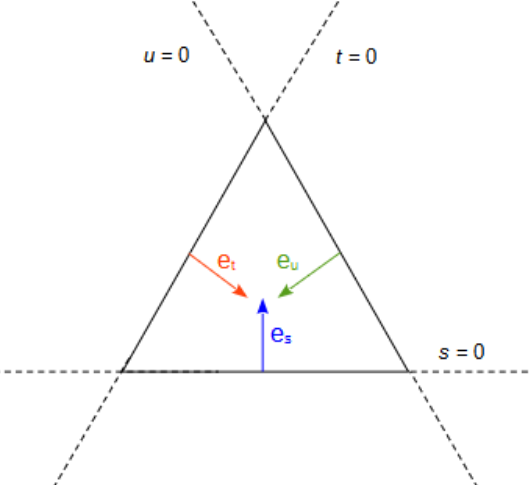
\includegraphics[width=0.45\textwidth]{immagini/fig_mandelstam.png}
            \caption{Piano di Mandelstam}%Ragazzi non ne ho idea è più comprensibile il corso di Greco.}
            \label{fig:mandelstam}
        \end{figure}
        I confini di questo triangolo sono dati dalle linee \( s = 0 \), \( t = 0 \) e \( u = 0 \), come mostrato. Il vertice superiore del triangolo corrisponde a \( t = u = 0 \), quindi, dalla equazione precedente, vediamo che l'altezza del triangolo è \( M \). Sebbene siano necessari solo due vettori unitari per specificare una posizione in questo piano, è consuetudine definire tre vettori unitari \( \hat{e}_s \), \( \hat{e}_t \) e \( \hat{e}_u \), ciascuno dei quali è perpendicolare alla rispettiva linea zero, come mostrato in \autoref{fig:mandelstam}. Visto che l'angolo tra due di questi versori è sempre $\frac23\pi$, abbiamo 
          \begin{equation*}
          \hat{e}_i\cdot\hat{e}_j=\cos\frac23\pi=-\frac12 \qquad i\neq j
          \end{equation*}
        Per qualche motivo oscuro vogliamo esprimere ${\hat e_i}$ in funzione di $\hat x$ e $\hat y$. Notiamo subito che $\hat e_s=\hat y$. Invece $\hat e_u$ ha un angolo pari a $\frac23\pi+\frac\pi2=\frac76\pi$ rispetto all'asse $\hat x$, dunque $\hat e_u=(-\frac{\sqrt3} 2,-\frac12)$. Infine $\hat e_t$ sta a $-\frac\pi6$ rispetto all'asse $\hat x$, quindi $\hat e_t=(\frac{\sqrt3}2,-\frac12)$. Queste relazioni possiamo invertirle e ricavare $\hat x$ e $\hat y$ in funzione di $\hat e_i$. Sempre per lo stesso oscuro motivo, la prof ci tiene a dire che le regioni fisicamente permesse sono quelle fuori dal triangolo e comprese tra le linee che fuoriescono da ciascun angolo. Per esempio la regione permessa di $s$ sta sopra. IO credo sia dovuto a questo: quando siamo nella retta parallela all'asse $x$ e passante per il vertice in alto, abbiamo  $s=4m^2,t=u=0$. Quindi se andiamo "sopra", $s>4m^2$ e $t,u<0$. Ok però così non ha senso che non si possa stare anche dentro il triangolo ok ci rinuncio. 
        \item c'è una parte poco chiara servirebbero slide.
        \item A cosa servono? Due sono indipendenti, la terza no e in base al processo che abbiamo esprimiamo le sezioni d'urto in funzione di una variabile piuttosto che di un'altra. Consideriamo un processo $X$ indipendente (forse senza polarizzazione?) da $\varphi$, allora 
        \begin{equation*}
        \dv{\sigma_X}{\Omega}=\frac1{2\pi}\dv{\sigma_X}{\dd{\cos\vartheta}}=\frac s{4\pi}\dv{\sigma_X}{t}\qquad \text{perché }t=-\frac s2\qty(1-\cos\vartheta)
        \end{equation*}
        Per $m^2\ll s$ la sezione d'urto dipende dal modulo quadro dell'elemento di matrice del processo
        \begin{equation*}
        \dv{\sigma_X}{t}=\frac{\abs{M_X}^2}{16\pi s^2}
        \end{equation*}
        In base al processo che considero, avrò una espressione diversa.
        \item Definizione di sezione d'urto, al solito probabilità di interazione quando il proiettile entra in regione unitaria di volume con un target. Considerimo un fascio di $N_b$ particelle contro uno strato $\dd l$ del target con $N_T$ particelle in volume $V$. Indicando con $n_T=\dd N_T/V$ la densità del target, abbiamo che $\dd{N_b}\propto N_b n_t\dd{l}$. 
        \begin{equation*}
        \dv{\sigma}{\Omega }=\pdv{\sigma}{\cos\vartheta}{\varphi}\underset{\text{Non dipende da } \varphi}{\Longrightarrow}\frac1{2\pi}\dv{\sigma}{\cos\vartheta}
        \end{equation*}
        \begin{equation*}
        \dv{\sigma}{\vec p}=\frac{\dd[3]{\sigma}}{\dd{p_x}\dd{p_y}\dd{p_z}}=\frac{\dd[3]{\sigma}}{p_T\dd{p_T}\dd{p_L}\dd{\varphi}}\Longrightarrow \text{slide}
        \end{equation*}
        Non lo so perchè ho scritto ciò\footnote{Ho chiesto a \href{https://chatgpt.com/share/672ba43f-ff50-800b-bc35-8bc186c6df2a}{ChatGPT} di spiegare i passaggi e sotto c'è lo jacobiano  (ovviamente mi dicono dalla regia, cervello mode: off) da $(x,y,z)\to(p_T,\varphi,p_L)$ con $p_T=\sqrt{p_x^2+p_y^2},\varphi=\tan^{-1}\qty(\frac{p_y}{p_x}),p_L=p_z$}.
        \item Una cosa da attenzionare è che la sezione d'urto bisogna precisare a cosa è riferita. Consideriamo $ab\to cX$. Se mi interessa solo sapere come è prodotto $c$ e non mi interessa da cosa è accompagnato, è una sezione d'urto \textit{inclusiva} $\sigma(ab\to cX)$ e devo considerare tutti i processi che lo producono. Se invece sono interessato ad un canale ben preciso, avrò la sezione d'urto \textit{esclusiva}. La somma di tutte le sezioni d'urto esclusive darà quella inclusiva. Quindi se $\sigma\_{inc}\ll\sigma\_{tot}$ allora posso esplicitare la probabilità di produrre $c$:
        \begin{equation*}
        \probP(c)=\frac{\sigma\_{inc}(ab\to cX)}{\sigma\_{tot}(ab)}
        \end{equation*} 
        Se invece $\sigma\_{inc}\approx\sigma\_{tot}$ allora quel rapporto fornisce il numero di $c$ prodotti nello stato finale. 
        \item In base al contesto posso esplicitare o meno se si tratta di sezione d'urto inclusiva/esclusiva. Ad esempio in LHC si lavora per la produzione di Higgs, quindi è sottointeso che la sezione d' urto sia inclusiva.
        \begin{equation*}
        \sigma\_{Higgs}\qty(\text{LHC},8\,\TeV)=\sigma\_{inc}\qty(pp\to Hx,\sqrt s =8\,\TeV)\approx22.3 \text{ pb}
        \end{equation*}
        \begin{equation*}
        \sigma\_{tot}\qty(pp,\sqrt s=8\,\TeV)=101.7\pm2.9\text{ mb}
        \end{equation*}
        Quindi ci sono 10 ordini di grandezza di differenza (pico $=10^{-12}$, milli $=10^{-3}$). Il rapporto ci dà la probabilità di produrre il bosone di Higgs:
        \begin{equation*}
            \probP(\text{Higgs @ LHC})=2\cdot 10^{-10}
        \end{equation*}
        Vediamo un altro esempio.
        \begin{equation*}
            \sigma\_{inc}\qty(pp\to\pi^0X,\,p\_{LAB}=24\,\GeV)=53.5\pm3.1\,\text{mb}
        \end{equation*}
        \begin{equation*}
            \sigma\_{to}\qty(pp,\,p\_{LAB}=24\,\GeV)=38.9\,\text{mb}
        \end{equation*}
        In questo caso il rapporto dà il numero. La probabilità la abbiamo solo se la frazione è \textit{molto} piccola.
        \item La sezione d'urto inoltre è legata alla matrice del processo, al fattore di spazio delle fasi $\qty(\frac{2\pi}\hbar\rho(E))$ e al rapporto tra elemento di volume e velocità della particella incidente tramite la seconda regola d'oro di Fermi.
        \begin{equation*}
            \sigma=\frac{WV}{v_b}=\frac{2\pi}\hbar\abs{M\_{if}}^2\rho(E)\frac V {v_b}
        \end{equation*}
        Con la teoria abbiamo questa espressione della sezione d'urto. Noi con la teoria accediamo a $\abs{M\_{if}}^2$ mentre sperimentalmente abbiamo numero di eventi in un determinato canale e poi si confronta.
        \item Nel caso di stati eccitati il decadimento è esponenziale $N(t)=N_0e^{-t/\tau}$ con $\tau$ tempo di vita medio del processo, con al solito $\Gamma\propto\frac1\tau$. Se $\tau$ è piccolo, l'energia a riposo (o massa) di uno stato non è unica (non è una delta di Dirac) ma varia attorno ad un valore centrale. La funzione che descrive la distribuzione di energia che lo stato può assumere è una lorentziana:
        \begin{equation*}
            \abs{\tilde\psi(E)}^2=\frac1{2\pi}\frac{\abs{\psi_0}^2}{(E-E_0)^2+\Gamma^2/4}
        \end{equation*} 
        che però in questo contesto fisico chiamiamo formula di Breit-Wigner (la si ricava facendo la trasformata di Fourier di $\psi(t)=\psi_0e^{-i(E_0-i\Gamma/2)t}$). La larghezza a metà altezza della lorentziana è proprio $\Gamma$ ed è la larghezza di decadimento. Questa formula è importante perché la Breit-Wigner appare ogni volta che abbiamo processi con risonanze, e dal picco troviamo la massa e dalla larghezza del picco troviamo la larghezza di decadimento (o tempo di vita medio).
        \item Consideriamo un processo con step intermedio $ab\to R\to X$. Allora abbiamo la formula ($J_R$ momento angolare totale della risonanza mentre $s_a,s_b$ spin delle particelle iniziali)\footnote{Sto 16 nella formula dopo non lo capisco, dovrebbe essere un 4. Purtroppo la campionessa non passa le slide quindi non posso controllare se è colpa mia.}
        \begin{equation*}
            \sigma(ab\to R\to X, E\_{cm}=\sqrt s)=\frac\pi{\abs{p_{ab}}^2}\underbrace{\frac{2J_R+1}{(2s_a+1)(2s_b+1)}}_{\begin{subarray}{c}
                \text{molteplicità di stati di spin}\\
                \text{ e momento angolare}
             \end{subarray}}\underbrace{\frac{\Gamma_{ab}\Gamma_X}{(\sqrt s-M_R)^2+\Gamma_R^2/4}}_{\text{Breit-Wigner}}\approx
        \end{equation*}
        \begin{equation*}
            \underset{\begin{subarray}{c}
            \text{trascuro masse}\\
            s\approx \abs{p_{ab}}^2
         \end{subarray}}{\approx}\frac{16\pi}s \frac{2J_R+1}{(2s_a+1)(2s_b+1)}\frac{\Gamma_{ab}}{\Gamma_R}\frac{\Gamma_X}{\Gamma_R}\frac{\Gamma_R^2/4}{(\sqrt s-M_R)^2+\Gamma_R^2/4}
        \end{equation*}
        quindi la si scrive in termini del branching ratio BR con i rapporti delle larghezze di decadimento. Applichiamola ad un caso specifico:
        \begin{equation*}
            \sigma(e^+e^-\to J/\psi\to\mu^+\mu^-)=\frac{16\pi}s\frac{3}{4}\frac{\Gamma_{e^+e^-}}{\Gamma_{J/\psi}}\frac{\Gamma_{\mu^+\mu^-}}{\Gamma_{J/\psi}}\frac{\Gamma_{J/\psi}^2/4}{(E-M_{J/\psi})^2+\Gamma_{J/\psi}^2/4}=
        \end{equation*}
        \begin{equation*}
            =\frac{12\pi}s\text{BR}({J/\psi\to e^+e^-})\text{BR}({J/\psi\to\mu^+\mu^-})\frac{\Gamma_{J/\psi}^2/4}{(E-M_{J/\psi})^2+\Gamma_{J/\psi}^2/4}
        \end{equation*}
        Da notare che non si conosceva nulla sulla $J/\psi$, né momento angolare né massa. Da fit si ricavarono entrambi. È importante sottolineare che la presenza di questo step intermedio è dovuta al fatto che sperimentalmente si osserva una risonanza, da ciò deduciamo che non sta semplicemente avvenendo $e^+e^-\to\mu^+\mu^-$. 
        \item Ci sono diverse formule di Breit-Wigner semi-empiriche o \textit{ispirate}. Ne abbiamo già viste due, ma possiamo anche averne una considerando $M_R\gg\Gamma_R$ e nego la dipendenza da $s$ (?); oppure in regime relativistico un'altra formula. 
        \item In generale quando faccio una misura io \textbf{non} ottengo mai la vera larghezza di decadimento, ma una convoluzione della larghezza intrinseca del decadimento e l'efficienza del rivelatore. 
        \item Quando abbiamo grandi numeri, consideriamo la distribuzione gaussiana mentre con piccoli numeri può essere binomiale o altro a seconda dei casi. Per scoprire una nuova particella consideriamo la distribuzione di Gauss e quando siamo distanti dal valore atteso: quando ci troviamo tra 3 e 5 deviazioni standard, si conclude che abbiamo \textit{osservato} qualcosa di nuovo. Se siamo oltre 5 deviazioni standard, si conclude che abbiamo \textit{scoperto} qualcosa di nuovo. Ovviamente è una convenzione.
        \item La forma della curva quando si osserva una risonanza è la \textit{Voigt} che tiene conto di larghezza intrinseca e risoluzione del rivelatore. Non ha una forma analitica ma solo integrale (di gaussiana per lorentziana).
\end{itemize}